\chapter{Machine Learning per l'Anomaly Detection}

In questo capitolo viene esposto il flusso che abbiamo seguito e le scelte effettuate per la realizzazione di quest'analisi empirica.

\section{Esplorazione dei Dataset}
Il primo approccio avviene tramite un approfondita esplorazione dei dataset reali disponibili, concentrandosi maggiormente su OPS\textunderscore SAT e NASA, entrambi con caratteristiche e peculiarità uniche, di interesse per il contesto satellitare.

Questi dataset sono stati presi in esempio, non solo per avere un confronto diretto con il repository di SpaceAI$^{\text{\cite{SpaceAI}}}$, ma anche per le sfide nell'ambito della rilevazione di anomalie, come la scarsa quantità di queste, i problemi relativi all'etichettatura e i dati che a volte possono mancare.

OPS\textunderscore SAT, permette un primo approccio molto più tranquillo, portando una struttura semplice, in modo che sia facile da comprendere e da utilizzare per lo sviluppo di nuovi algoritmi.
NASA, d'altro canto, è il dataset che rappresenta di più la realtà, portando dati più complessi, che sarà utilizzato come banco di prova più realistico.


\section{Flusso di Lavoro}
Il primo approccio, come abbiamo spiegato precedentemente, avviene con il dataset OPS\textunderscore SAT, dal quale, dopo aver validato tutti i risultati ottenuti dai modelli del relativo paper, abbiamo cercato di migliorare XGBOD, uno dei migliori modelli per capacità di rilevare le anomalie e velocità di esecuzione. Abbiamo effettuato test per trovare i migliori iperparametri basandoci sulle metriche e sul tempo di esecuzione.

Su OPS\textunderscore SAT siamo poi passati all'implementazione di ROCKET, apportando modifiche ai dati estratti per renderli compatibili ed utilizzabili con ROCKET.
Data la natura di ROCKET, che utilizza le serie temporali, siamo riusciti ad utilizzarlo come estrattore di caratteristiche per poi utilizzarle con un classificatore per ottenere i risultati voluti.
Come classificatori abbiamo utilizzato vari modelli, sia unsupervised che supervised, tra cui l'uso di una threshold in percentuale, utilizzando il 95° percentile dei punteggi di anomalia; ulteriori prove sono state effettuate con KNN, LogisticRegression, Ridge e RidgeClassifierCV che troviamo utilizzati anche nel paper di ROCKET$^{\text{\cite{paper_rocket}}}$.
Lo stesso processo è stato effettuato con ROCKAD utilizzando però come classificatore il modello proposto nel paper di riferimento$^{\text{\cite{rockad_paper}}}$, NearestNeighborOCC.

Partendo da OPS\textunderscore SAT siamo arrivati a NASA per ottenere una conferma dell'efficienza ed efficacia degli algoritmi.
In questo dataset, al contrario di OPS\textunderscore SAT, l'etichettatura dei dati di training non è presente potendo così utilizzare solo modelli unsupervised.
Anche per questo dataset c'è stata la necessità di rendere i dati compatibili per l'utilizzo.

Tutti i risultati ottenuti sono stati proposti in tabelle ordinate e analizzati per trarne le conclusioni, in rifermento soprattutto a ROCKET il quale è stato utilizzato per la prima volta come metodo per il rilevamento delle anomalie, valutandone così la vera potenza e efficienza.

\section{Misure di Valutazione}
Analizzeremo ora le metriche che ci permettono di valutare le prestazioni di un algoritmo allenato sui dati del training set e utilizzato come classificatore per il rilevamento delle anomalie quindi con i relativi pesi calcolati.

Utilizziamo le seguenti metriche, dalle quali trarremo le conclusioni sulle capacità di ciascun algoritmo: 
\begin{itemize}
    \item \textbf{Accuratezza}: rappresenta la percentuale di previsioni corrette (TP - True Positive) su tutti i casi possibili, tiene in considerazione anche i veri negativi (TN).
    Questa misura ci indica la percentuale dei dati riconosciuti correttamente. 
    
    \textit{Formula:}
        \begin{equation}
            \frac{TP+TN}{TP+TN+FP+FN}
        \end{equation}
    
    \item \textbf{Precisione}: rappresenta la percentuale di anomalie vere rilevate in confronto a tutte le anomalie segnalate.

    \textit{Formula:}
        \begin{equation}
            \frac{TP}{TP+FP}
        \end{equation}
    Nel nostro caso questa metrica è particolarmente importante, dato che un valore troppo basso significherebbe un'alta probabilità di avere falsi positivi, portando quindi uno spreco di banda ed energia per mandare i messaggi ed un allarme che richiede un intervento non necessario.

    \item \textbf{Recupero}: rappresenta la capacità di rilevare le anomalie tenendo in considerazione le anomalie reali. Questa misura è anche detta sensibilità.

    \textit{Formula:} 
    \begin{equation}
        \frac{TP}{TP+FN}
    \end{equation}
    Nel contesto dei satelliti questa metrica è cruciale dato che, con un valore basso avremo un grande numero di falsi negativi (FN), che senza intervento potrebbero portare a conseguenze molto gravi.
    
    \item \textbf{$\boldsymbol{F_1}$ score}: rappresenta una media armonica tra precisione e recupero dove il massimo si ottiene con il valore uno e il minimo a zero.

    \textit{Formula:}
    \begin{equation}
        F_1=\frac{2*TP}{2*TP+FP+FN}
    \end{equation}
    Questa metrica nel nostro caso è importante, infatti cerchiamo un buon compromesso tra precisione e richiamo, per non avere un alto numero, né di falsi negativi, né di falsi positivi. Questo porta ad un equilibrio tra precisione e capacità di rilevazione.

    \item \textbf{Coefficiente di correlazione di Matthews (MCC)}$^{\text{\cite{matthew}}}$: rappresenta una misura della qualità del modello con dati molto variabili.

    \textit{Formula:}
    \begin{equation}
        \frac{TP\cdot TN-FP\cdot FN}{\sqrt{(TP+FP)\cdot (TP+FN)\cdot(TN+TP)\cdot(TN+FN)}}    
    \end{equation}
    Questa misura è particolarmente indicata per il rilevamento delle anomalie, dato che concede la stessa importanza a veri positivi, falsi positivi, veri negativi e falsi negativi.

    \item \textbf{L'area sottesa alla curva ROC (AUC$_\text{ROC}$}$^{\text{\cite{ROC_google}}}$$^{\text{\cite{ROC}}}$): rappresenta il rapporto tra il tasso di veri positivi e il tasso di falsi positivi (Figura: \ref{fig:Curva ROC}).
    Questa permette di osservare come varia il richiamo in funzione della metrica di precisione. Può anche essere usato per scegliere il modello migliore tra due, guardando semplicemente l'area sottesa al grafico: quella con l'area più grande è generalmente quello migliore.

    \begin{figure}
        \centering
        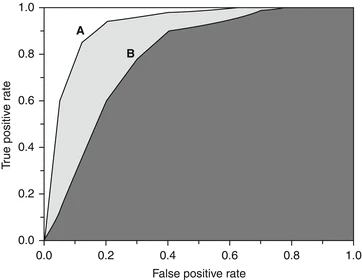
\includegraphics[width=0.5\linewidth]{images//Capitolo3/Curva ROC.png}
        \caption{Curva ROC}
        \label{fig:Curva ROC}
    \end{figure}
    
    \item \textbf{Area sottesa alla curva Precisione-Richiamo (AUC\textunderscore PR)}: rappresenta un semplice modo per sintetizzare le prestazioni generali di un modello, più alto è il valore più alto sarà il numero di predizioni corrette. La curva Precision-Recall è utile quando la classe positiva è rara, perché si concentra sulla capacità del modello di identificare correttamente i casi positivi, senza essere influenzata dai veri negativi.
\end{itemize}
In queste formule per il calcolo delle metrica abbiamo usato: TP per rappresentare i veri positivi, ossia i segmenti delle telemetrie correttamente identificati come anomalie; TN per i veri negativi, cioè segmenti correttamente identificati come nominali ossia regolari; FP per i falsi positivi, ossia i segmenti erratamente classificati anomalie e FN per i falsi negativi che rappresentano i segmenti erratamente classificati come non anomalie.
Tutte le metriche descritte possono assumere valori tra $[0,1]$, tranne MCC che assume valori tra $[-1,1]$.
Tutte le metriche però più si avvicinano ad uno e più il modello testato risulta efficace, rispetto ad uno con valori inferiori delle stesse.

Le metriche appena viste ci serviranno successivamente per valutare le capacità degli algoritmi avendo un metro di paragone unico per tutti i modelli.
Tra gli obbiettivi resta comunque cercare di non sovraccaricare il processore del satellite, mantenendo quindi la complessità del modello abbastanza bassa.
Nell'eventualità di una piccola perdita di efficacia, ma con un grande risparmio in complessità del modello, viene ovviamente premiata l'efficienza.
